%
%===============>>  Сорокин Модуль 6 <<=============
%=
\setmodule{5}

%BEGIN_FOLD % ====>>_____ Занятие 1 _____<<====
\begin{class}[number=1]
	\begin{listofex}
		\item Занятие 1
	\end{listofex}
\end{class}
%END_FOLD

%BEGIN_FOLD % ====>>_ Домашняя работа 1 _<<====
\begin{homework}[number=3]
	\begin{listofex}
		\item Найдите значение выражения: \( \dfrac{12 \sin{11\degree} \cdot \cos{11\degree}}{\sin{22\degree}} \)
		\item Найдите значение выражения: \( \dfrac{24 (\sin^2{17\degree} - \cos^2{17\degree})}{\cos{34\degree}} \)
		\item Найдите значение выражения: \( -4\sqrt{3}\cos{(-750\degree)} \)
		\item Найдите значение выражения: \( 2\sqrt{3}\tg{(-300\degree)} \)
		\item Найдите значение выражения: \( 24\sqrt{2}\cos{\left( -\dfrac{16\pi}{3}\right)}\sin{\left( -\dfrac{17\pi}{4} \right)} \)
		\item Найдите значение выражения: \( \dfrac{8}{\sin{\left(-\dfrac{27\pi}{4}\right)}\cos{\left(\dfrac{31\pi}{4}\right)}} \)
		
		\item Найдите \( 3\cos{a} \), если \( \sin{a}= - \dfrac{2\sqrt{2}}{3} \) и \(a\) принадлежит \( \left( \dfrac{3\pi}{2}; 2\pi \right) \)
		\item Найдите \( \dfrac{10\sin{6a}}{3\cos{3a}} \), если \( \sin{3a}=0,6 \)
		\item
		\begin{minipage}[t]{0.3\textwidth}
			На рисунке изображён график функции вида \(f(x)=ax-|bx+c|+d\), где числа \(a, b, c, d\) --- целые. Найдите корень уравнения \(ax+d=0\).
		\end{minipage}
		\begin{minipage}[c]{0.1\textwidth}
			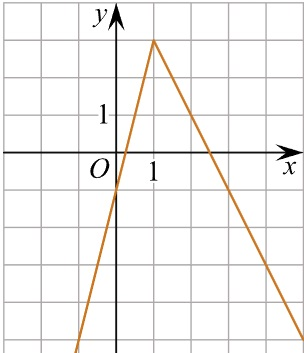
\includegraphics[align=t, width=\textwidth]{../../pics/G111M4C5-3.jpg}
		\end{minipage}
		\item 
		\begin{minipage}[t]{0.3\textwidth}
			На рисунке изображён график функции вида \(f(x)=\dfrac{x^2}{a}+bx+c\), где числа \(a, b, c\) --- целые. Найдите значение \(f(2,5)\).
		\end{minipage}
		\begin{minipage}[c]{0.12\textwidth}
			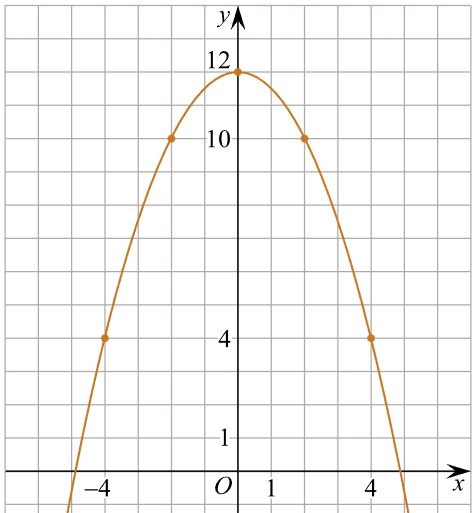
\includegraphics[align=t, width=\textwidth]{../../pics/KUZNETSOVM6H1-1.jpg}
		\end{minipage}
		\item Найдите корень уравнения: \( \log_2(4-x)=7 \)
		\item Найдите корень уравнения: \( \log_5(5-x)=\log_5{3} \)
		\item Найдите корень уравнения: \( \log_4(x+3)=\log_4(4x-5) \)
		\item Найдите корень уравнения: \( 2^{4-2x}=64 \)
		\item Найдите корень уравнения: \( 5^{x-7}=\dfrac{1}{125} \)
		\item Найдите корень уравнения: \( \left( \dfrac{1}{3} \right)^{x-8} = \dfrac{1}{9} \)
		\item Решите неравенство: \( (x^2-6x+8)(x-6) \le 0 \)
		\item Решите неравенство: \( (3x^2-5x+2)(2x-1)^2 \le 0 \)
		\item Решите неравенство: \( \dfrac{1}{x-1}+\dfrac{1}{2-x} \le 5 \)
		\item Решите неравенство: \( \dfrac{2x^2-2x+1}{2x-1} \le 1 \)
		\item Решите неравенство: \( \sqrt{x^2-5x+15} \le 3 \)
	\end{listofex}
\end{homework}
%END_FOLD

%BEGIN_FOLD % ====>>_____ Занятие 2 _____<<====
\begin{class}[number=2]
	\begin{listofex}
		\item Занятие 2
	\end{listofex}
\end{class}
%END_FOLD

%BEGIN_FOLD % ====>>_ Домашняя работа 2 _<<====
\begin{homework}[number=2]
	\begin{listofex}
		\item Домашняя работа
	\end{listofex}
\end{homework}
%END_FOLD

%BEGIN_FOLD % ====>>_____ Занятие 3 _____<<====
\begin{class}[number=3]
	\begin{listofex}
		\item Занятие 3
	\end{listofex}
\end{class}
%END_FOLD

%BEGIN_FOLD % ====>>_ Домашняя работа 3 _<<====
\begin{homework}[number=3]
	\begin{listofex}
		\item Домашняя работа
	\end{listofex}
\end{homework}
%END_FOLD

%BEGIN_FOLD % ====>>_____ Занятие 4 _____<<====
\begin{class}[number=4]
	\begin{listofex}
		\item Пусто
	\end{listofex}
\end{class}
%END_FOLD


%BEGIN_FOLD % ====>>_ Проверочная работа _<<====
\begin{exam}
	\begin{listofex}
		\item Проверочная
	\end{listofex}
\end{exam}
%END_FOLD